\chapter{Creazione del modello Simulink}

\section{Creazione del modello Simulink}
Prima di validare il set-up sperimentale costituito, è necessario verificare il corretto funzionamento del sistema tramite un modello Simulink.\\
Si è innanzitutto implementato la procedura di misurazione. Per semplificare la sua costruzione, si è considerato la velocità del motore di test costante.\\
Si assume anche che le componenti di corrente d-q seguano perfettamente il riferimento.\\
In seguito verrà realizzato il modello completo, considerando anche il motore controllato in velocità che trascina il motore di test.\\

\section{Controllo di corrente}
Per controllare il motore si è utilizzato un controllo PID proporzionale integrale. Si è implementato anche un sistema Feedforward per eliminare il cross-coupling.\\
Tutti i blocchi per il controllo di corrente sono stati realizzati nel discreto.
È importante notare come questo sia possibile perché il valore di induttanza da utilizzare per il FFW è fornita dal datsaheet. In un caso reale, in cui tale valore non sia noto, non è possibile eseguire tale procedura.\\
 I parametri del controllore PID sono stati tarati manualmente per evitare sovraelongazioni e oscillazioni di corrente.\\
I controllori PID sono provvisti anche di anti-windup per evitare la saturazione dell'azione integrale.






\begin{figure}
\centering
    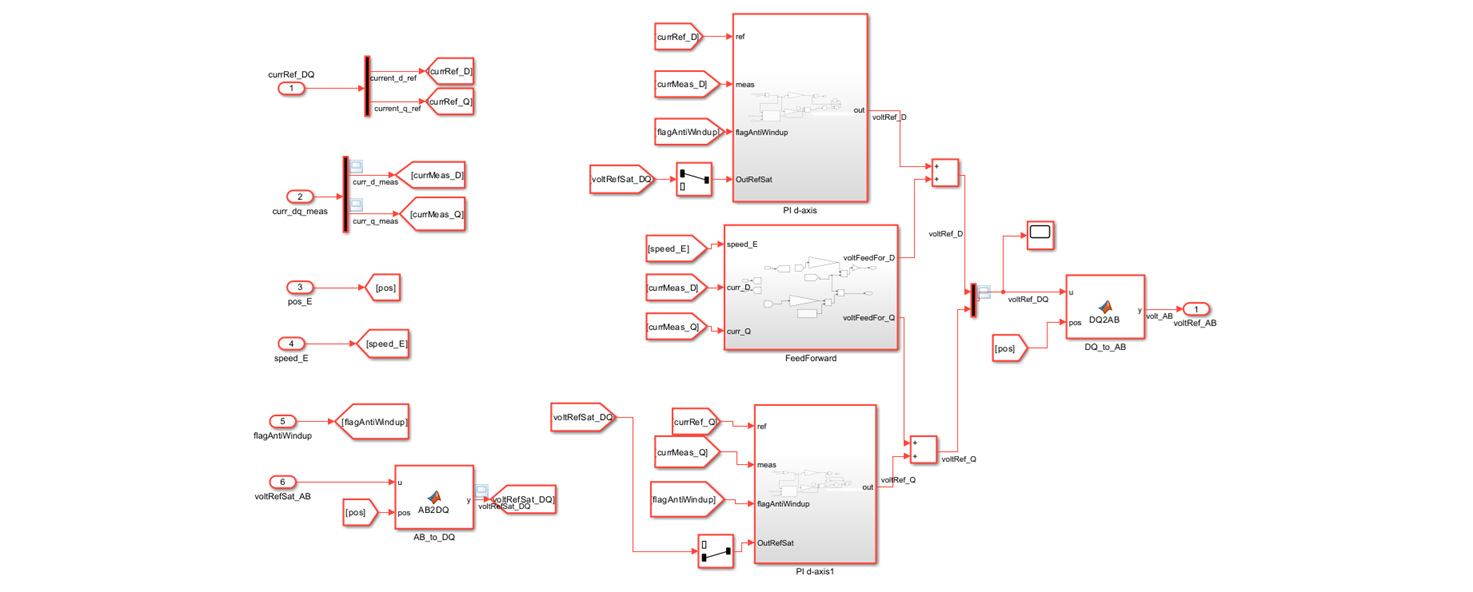
\includegraphics[height=8 cm]{immagini/immagini_motore/controllo_corrente_motore.png}
    \caption{Blocchi di controllo di corrente del motore.} 
    \label{fig:controllo_corrente_motore}
\end{figure}

\section{Implementazione della macchina a stati}

La procedura di misurazione può essere suddivisa in cin cinque fasi principali: 
\begin{enumerate}
    \item Fase di stima della resistenza di statore
    \item Fase di variazione di corrente
    \item Fase di attesa dello zero meccanico
    \item Fase di misurazione
    \item Conclusione della procedura
\end{enumerate}
Per gestire le varie fasi della procedura è stato utilizzato il blocco \texttt{Stateflow} di \texttt{SIMULINK}.\\
Per tenere traccia dello stato di avanzamento della procedura, il blocco \texttt{Stateflow} utilizza il contatore \texttt{stato}. Tale variabile è iizializzata a  0 e viene incrementata di 1 al termine di ogni fase di variazione di corrente e misurazione. Raggiunto il valore 6, il sistema di controllo porta le correnti a 0 e termina l'operazione.\\\
Uno schema della procedura è riportato in Figura \ref{fig:flowchart_stati}.

\begin{figure}
\centering
    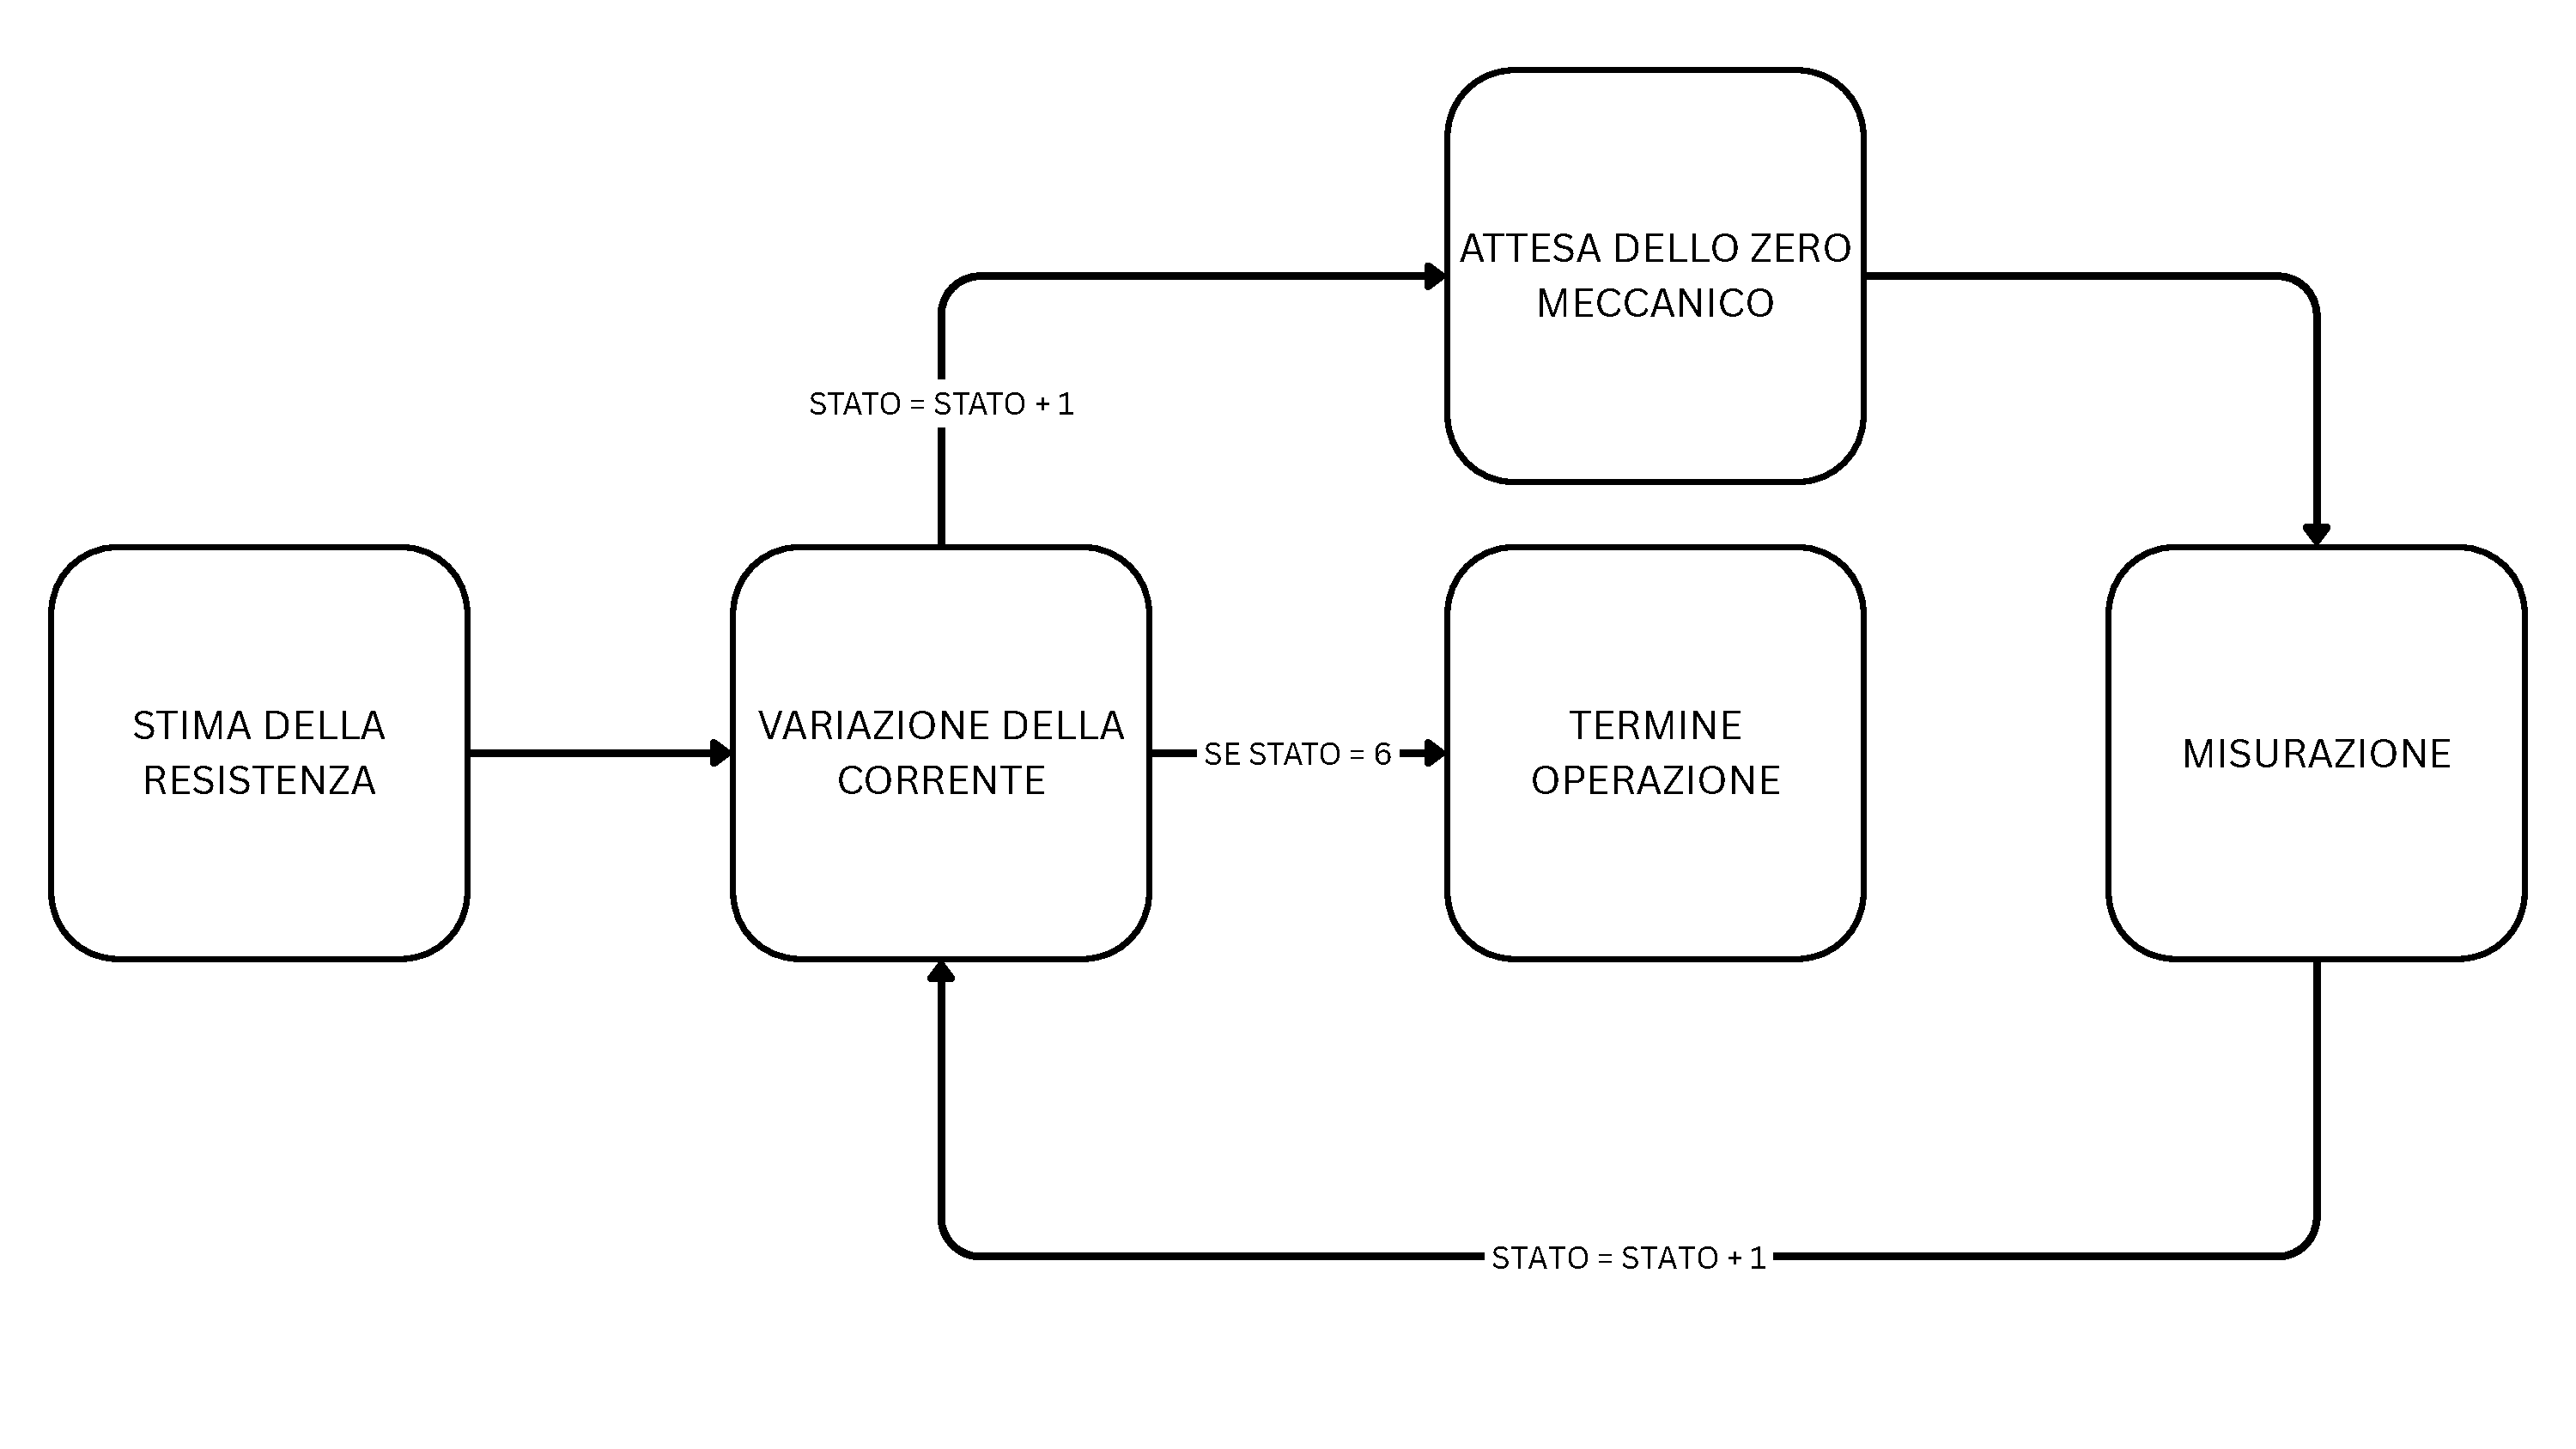
\includegraphics[height=8 cm]{immagini/immagini_motore/flowchart_stati.pdf}
    \caption{Schema della procedura di misurazione.} 
    \label{fig:flowchart_stati}
\end{figure}

\subsection{Fase di stima della resistenza di statore}
Le stime del flusso per ogni coppia di correnti vengono eseguite in successione. Di conseguenza, all'avvio di ogni sessione di raccolta dati, si riscontra una temperatura diversa da quella di partenza e quindi anche una resistenza differente.\\
Per stimare la resistenza, all'inizio di ogni sessione di misurazione viene applicato un segnale di corrente $i_d$ pari a metà della corrente nominale \cite{Gierczynski}. \\
Come nella fase di variazione di corrente, anche in questa fase si raggiunge il valore desiderato tramite una rampa di corrente. Anche in questo caso la pendenza è pari a $2 \ A/s$.\\
La corrente $iq$ viene mantenuta nulla per la durata dell'impulso $id$.\\
Dato che la corrente $iq$ è pari a 0, anche il flusso $\lambda_q$ risulta nullo.\\
In questo modo risulta che:


\begin{equation}
    u_d = R_{s}\cdot i_d
\label{eq:res_iq_null}
\end{equation}
\begin{equation}
    u_q = \omega_{me}\cdot\lambda_d(i_d,i_q,\theta_m)
\end{equation}
Atteso l'esaurimento del transitorio, vengono prelevati 100 campioni di corrente e tensione.\\
Dalla \ref{eq:res_iq_null} si può ricavare una stima della resistenza:
\begin{equation}
\hat{R}_{ph} = \overline{u}_d / \overline{i}_d , 
\end{equation}




\subsection{Fase di variazione di corrente}

Come prima cosa viene verificat loo stato del sistema.
Se il contatore ha raggiunto il valore di 6, significa che il sistema ha completato la procedura di misurazione per un determinato punto di lavoro e deve terminare l'operazione.\\
Inanzitutto si impone i valori di corrente $i_d$ e $i_q$ da raggiungere. Tali valori identificano un punto della griglia nella procedura completa.
I riferimenti di corrente $i_q^*$ e $i_d^*$ variano linearmente fino a raggiungere il valore desiderato. \\
Si è fissata una pendenza della rampa di corrente pari a $2 \ A/s$. Dato che il tempo di campionamento è di $10^{-4}$ s, l'incremento di corrente ad ogni passo di esecuzione è pari a $2\cdot10^{-4}$ A.\\
Una volta che la differenza tra il riferimento di corrente e il valore desiderato è inferiore all' incremento di corrente, il riferimento di corrente viene fissato al valore desiderato.\\ 
Senza questa accortezza, la corrente di riferimento potrebbe non raggiungere il valore desiderato.\\
La scelta della pendenza della rampa è significativa in quanto influenza la durata della procedura di misurazione. Tuttavia, una pendenza troppo elevata può portare a oscillazioni della corrente e quindi a una stima del flusso non corretta.\\
Una volta raggiunto il valore desiderato viene attivato un flag che permette il passaggio allo stato successivo.\\


\subsection{Fase di attesa dello zero meccanico}
Prima di iniziare la fase di misurazione, è necessario attendere che la posizione meccanica del rotore sia pari a 0°.\\
In questo modo, infatti è garantito che tutte le misurazioni vengano eseguite a partire dalla stessa posizione meccanica.\\
Per evitare di iniziare a campionare quando il transitorio di corrente non si è ancora esaurito si è deciso di attendere un tempo di 0.2 s prima di iniziare la fase di misurazione.\\
Se il rotore raggiunge la poszione meccanica di 0° prima che siano trascorsi 0.2 s il sistema attende fino a quando il motore non raggiunge nuovamente tale posizione meccanica e il tempo di attesa è trascorso.\\

\begin{figure}
\centering
    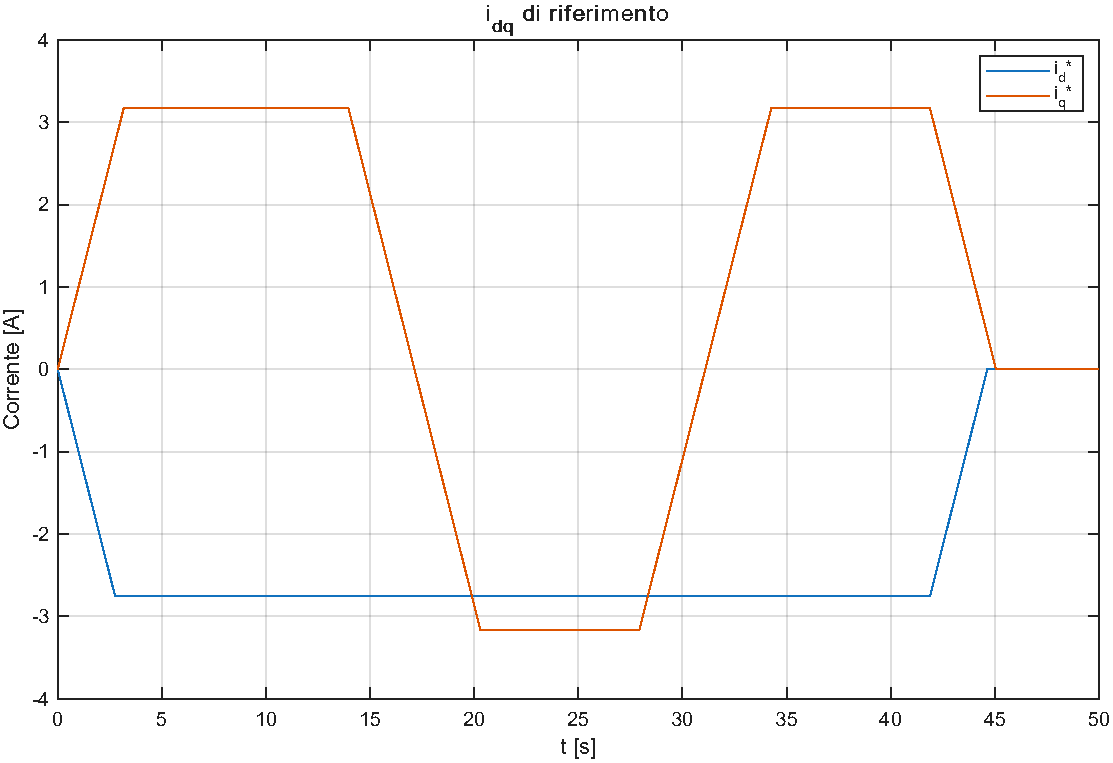
\includegraphics[height=8 cm]{immagini/procedura_misurazione/Curr_ref_proc.pdf}
    \caption{Andamento della corrente di riferimento ( $i_d$ = -2.692, $i_q$ = 3.224 A)}
    \label{fig:Curr_ref_proc}
\end{figure}

\subsection{Fase di misurazione}
In questa fase le misure di corrente e tensione vengono caricate in un vettore di dati.\\
I dati inviati al workspace di MATLAB sono la tensione, la corrente e la poszione meccanica. I dati di corrente e tensione sono espressi secondo il sistema $abc$ e verranno poi trasformati nel sistema $\alpha\beta$.\\
Per attivare il caricamento dei dati nel vettore apposito, viene attivato un flag che abilita il blocco "Enabled Subsystem" di Simulink.\\
La procedura di misurazione termina quando il rotore completa un giro meccanico.\\
A ogni passo di esecuzione, viene calcolata la differenza tra la posizione attuale e quella precedente. Questo valore viene somamto a un contatore che permette di registrare la distanza angolare percorsa dal rotore.\\
Per separare le misurazioni di corrente, posizione e tensione avvenute nelle avrie fasi, al termine di una misurazione viene aggiunto un elemento NaN al del vettore di dati.\\
Una volta che il contatore raggiunge il valore di $360^{\circ}$, il sistema transita allo stato successivo e disabilita il blocco "Enabled Subsystem".\\


\subsection{Conclusione della procedura}

Una volta che il sistema ha effettuato l'ultima misurazione (M2), il sistema transita nuovamente allo stato di variazione di corrente. Il contatore \texttt{stato} ha raggiunto il valore 6, quindi le correnti di target vengono impostate a 0.\\
Dopo che entrambe le correnti hanno raggiunto il valore nullo, la simulazione termina dopo 1 s per attendere l'esaurimento del transitorio.\\
Il blocco \texttt{Stateflow} infine attiva un flag per teminare la simulazione.\\


\subsection{Andamento del segnale di corrente $dq$}
Per realizzare una mappa di flusso precisa, è necessario che, durante la fase di misura, la corrente rimanga il più possibile costante.\\
Si può notare in Figura \ref{fig:Curr_ref_proc_tot_stat} come, a regime, la corrente di statore oscilli intorno al valore di riferimento. Tuttavia, tale oscillazione risulta ininfluente e non incide sulla stima finale.\\
In quanto il flusso magnetico è influenzato dalla posizione, ad alta velocità il controllo risulta complesso. Esso, infatti, risulta affetto da oscillazioni significative che portano a una distorsione del segnale del flusso stimato. Il disturbo sul controllo di corrente è evidente in Figura \ref{fig:Curr_ref_proc_tot_5_rads}, dove la velocità di test imposta è di 5 rad/s.



\begin{figure}
\centering
    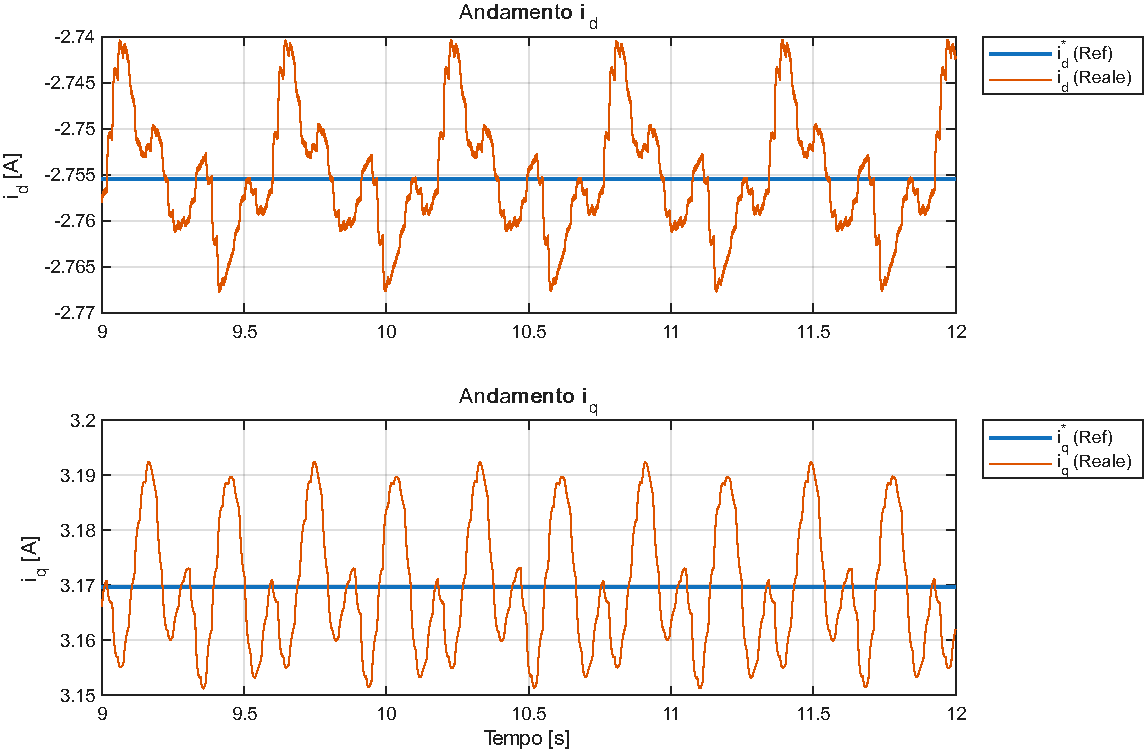
\includegraphics[height=8 cm]{immagini/procedura_misurazione/Curr_ref_proc_tot_stat.pdf}
    \caption{Oscillazione della corrente rispetto al riferimento ( $i_d$ = -2.692, $i_q$ = 3.224 A)}
    \label{fig:Curr_ref_proc_tot_stat}
\end{figure}

\begin{figure}
\centering
    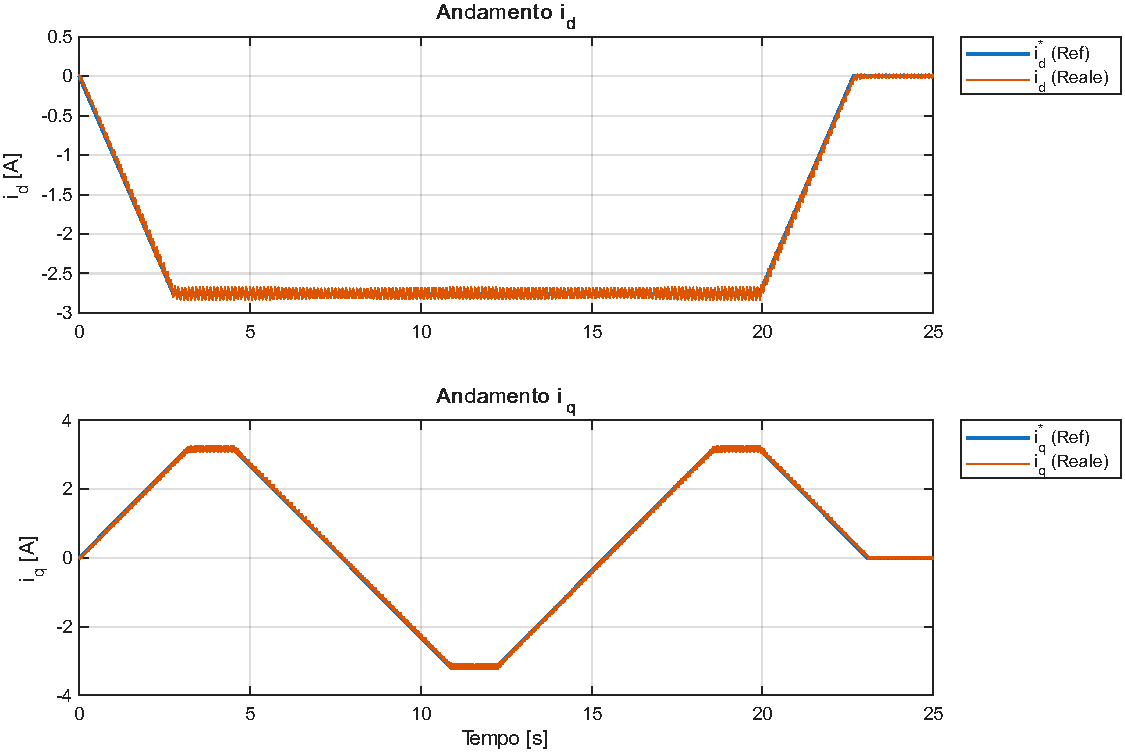
\includegraphics[height=8 cm]{immagini/procedura_misurazione/Curr_ref_proc_tot_5_rads.pdf}
    \caption{Andamento della corrente dq @ $\omega_m = 5\ rad/s$}
    \label{fig:Curr_ref_proc_tot_5_rads}
\end{figure}


 



\section{Procedura di campionamento}
I dati vengono campionati a una frequenza di 10 KHz, la stessa dell'inverter. La risoluzione dei sensori scelta è di $1\ mA$ per il sensore di corrente, $10 \ mV$ per il sensore di tensione e $5.49 \cdot10^{-3}$ gradi per il sensore di posizione.\\
Le grandezze di tensione, corrente e posizione meccanica costituiscono i segnali di ingresso per il blocco Stateflow di MATLAB. In tale blocco viene implementata sia la generazione del vettore di corrente, sia la gestione dei dati da inviarre al workspace di MATLAB.\\
Inizialmente, durante la fase di variazione della corrente e di attesa venivano salvati degli elementi NaN all'interno del vettore di output. Tuttavia, questo aumenta la dimensione del vettore di output.\\
Per ovviare a questo problema, si è deciso di salvare solo i dati della fase di misura, eliminando quelli della fase di variazione della corrente.\\
Per implementare questa proceura si è utilizzato il blocco "Enabled Subsystem" di Simulink.

\section{Elaborazione dati}
L'elaborazione dei dati raccolti avviene tramite un algoritmo MATLAB. Tale algoritmo, come la procedura di misurazione, può essere suddivisa in diverse parti:
\begin{enumerate}
 \item Preparazione dei dati per l'elaborazione tramite l'algoritmo di stima.
 \item Stima del flusso magnetico $\alpha\beta$ tramite l'integrazione della forza contro-elettromotrice.
 \item Trasformazione del flusso magnetico nel sistema di riferimento $dq$.
 \item Applicazione della formula per la stima del flusso magnetico, utilizzando i dati raccolti nelle tre fasi di misurazione (M1,G,M2)
\end{enumerate}

\subsection{Preparazione dei dati}
Per la trasformazione da $\alpha\beta$ a $dq$ è necessario disporre della posizione elettrica $\theta_e$ del rotore.\\
Dato che si tratta di un motore sincrono, tale grandezza è legata alla posizione meccanica del rotore tramite la seguente relazione:

\begin{equation}
\theta_e = {p}\cdot\theta_m
\end{equation}

dove $p$ è il numero di coppie polari del motore.\\
Per applicare la formula di integrazione i vettori di tensione $v_{abc}$ e corrente $i_{abc}$ misurati devono essre espressi secondo il sistema di riferimento $\alpha\beta$.\\ 
Per far ciò, si applica la trasformazione di Clarke sui dati raccolti per ogni fase di misurazione $y$:
\begin{equation}
\boldsymbol{v_{\alpha\beta}}{k} = \frac{2}{3} \cdot 
\begin{bmatrix} 
1 & -\frac{1}{2} & -\frac{1}{2} \\ 
0 & -\frac{\sqrt{3}}{2} & \frac{\sqrt{3}}{2} 
\end{bmatrix} \cdot \boldsymbol{v}_{abc,k}^{y}
\label{eq:eq14}
\end{equation}
\section{Elaborazione dati}
Una volta raccolti i dati essi vengono elaborati tramite un algoritmo \texttt{MATLAB}. Questo algoritmo implementa la procedura illustrata nel Paragrafo \ref{sec:stima_flusso}. I dati vengono quindi espressi secondo il sistema di riferimento $\alpha\beta$ . Si sottrae la componente resistiva alla tensione di Bus per ottenere la componente di forza contro-elettromotrice. 
Si integra la forza contro-elettromotrice e la si somma al valore del flusso all'istante iniziale.\\
A questo punto si esprime il flusso secondo il sistema $dq$. Dato che è necessario esprimere il flusso in funzione della posizione elettrica, i dati vengono riordinati a seconda della posizione elettrica. Nel caso in cui più dati siano associati alla stessa posizione elettrica si esegue una media dei valori di flusso.\\
A questo punto è possibile creare una funzione interpolatrice per confrontare i risultati ottenuti con il flusso reale, derivato dalle mappe dirette.



\subsection{Scelta della velocità meccanica del motore}
È poi necessario scegliere una velocità di rotazione del motore adeguata.\\
Una velocità troppo bassa porta a una maggiore influenza delle perdite nel ferro e nel magnete permanente, compromettendo una corretta stima del flusso. Tuttavia, una velocità elevata rende più difficile misurare il flusso per ogni posizione meccanica del motore. \\Ciò è dovuto al fatto che il tempo di campionamento di 10 KHz permette di misurare la posizione ogni 0.1 ms. Se la velocità è elevata, in tale intervallo di tempo lo spostamento del motore può superare la risoluzione del motore IPM sotto test ($5.493 \cdot 10^{-5} rad$).\\
Per ottenere una mappatura completa del flusso a seconda della posizione in un solo giro meccanico è necessario rispettare il seguente vincolo sulla velocità meccanica del rotore $\omega_M$:
\begin{equation}
\omega_M<\frac{\Delta_M}{T_s}  
\end{equation}
Nel caso del motore di test che abbiamo scelto il vincolo sulla velocità meccanica risulta:
\begin{equation}
\omega_M<0.958\ rad/s)
\end{equation}
\subsection{Trade-off sulla velocità del rotore}
Incrementare la velocità richiede necessariamente una sessione di misura più estesa o, in alternativa, il declassamento del dettaglio della mappatura.
Per esempio si potrebbe decidere di far ruotare il motore a una velocità tale che lo spostamento del motore in un intervallo di campionamento equivalga al doppio della risoluzione angolare ed effettuare due misurazioni. \\
Con questo metodo, è possibile recuperare il dettaglio originario effettuando due acquisizioni sfasate; in tal modo, il tempo complessivo di misura rimarrebbe invariato.\\
Tuttavia, in questo caso, la posizione del rotore in corrispondenza della quale iniziare la misurazione non è più ininfluente. È indispensabile che la seconda misurazione inizi con uno sfasamento di una tacca rispetto alla prima.



\begin{comment}
\subsection{Elaborazione dei dati ottenuti}
Una volta calcolato l'integrale della differenza tra la tensione misurata ai terminali e la tensione resistiva ($V_{\alpha \beta}-R_sI_{\alpha\beta}$), i dati ottenuti vengono filtrati con un filtro passa-alto.\\
L'obiettivo di quest'ultima operazione è:
\begin{itemize}
    \item Eliminare la componente DC: eliminare offset costanti che causerebbero una deriva del segnale.
    \item Riduzione dei fenomeni spuri: attenuare disturbi a bassa frequenza e anomalie di misura.
\end{itemize}

Per progettare il filtro passa-alto si è stata implementata la seguente equazione:

\begin{equation}
    y[k] = \alpha y[k-1] + \alpha (x[k] -x[k-1])
\end{equation}

Il parametro $alpha$ si ottiene a partire dalla frequenza di taglio di un equivalente filtro passa-alto in continua. Tale frequenza di taglio deve essere necessariamente inferiore rispetto alla frequenza della prima armonica del flusso magnetico $d$ e $q$. La fondamentale a di entrambi i flussi è centrata in:
\begin{equation}
    f_0 = \frac{w_m\cdot12}{2\pi} = 1.71\ Hz
\end{equation}
Per rispettare questo vincolo è stata scelta una frequenza di taglio di 1 Hz.
\end{comment}




